Para realizar la pantalla de supervisión, control y adquisición de datos operador se utilizó el software iFix perteneciente al grupo \textbf{General Electric}.

El sistema SCADA creado (Figura \ref{fig:scada1}) se dividió en las siguientes secciones:
\begin{itemize}
	\item Esquemático del circuito hidráulico físico con las variables de presión y caudal en tiempo real.
	\item Valores de funcionamiento del motor obtenidos por el variador de velocidad.
	\item Alarmero, dónde se observa de forma visual valores críticos alcanzados en el sistema.
	\item Indicador de modo de funcionamiento físico o remoto.
	\item Modo de control a lazo abierto o lazo cerrado.
	\subitem Para el modo de lazo cerrado se creó una ventana individual para cada sistema de presión y caudal.
	\item Pantalla para observar gráficos en tiempo real dónde se divide según la variable a observar, con botones para abrir el control PID del sistema.
	\item Pantalla donde se observa datos históricos y se puede generar un archivo \textit{.txt} con la información de la variable elegida en un determinado período de tiempo.
\end{itemize} 

\begin{figure}[htb]
	\centering
	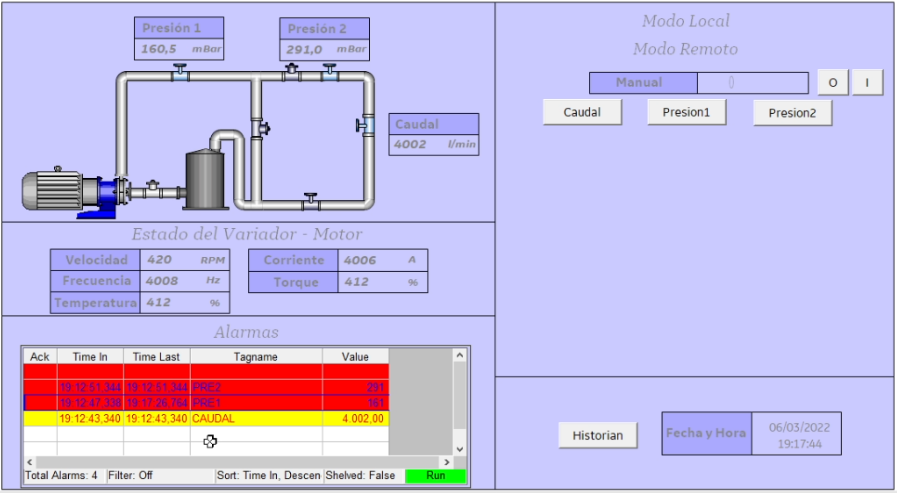
\includegraphics[width=0.9\linewidth]{scada1.png}
	\captionof{figure}{Pantalla SCADA}
	\label{fig:scada1}
\end{figure}


\subsubsection{Configuración driver Modbus}
Para realizar la configuración de cada ícono de la pantalla SCADA con su respectiva variable, se debió crear un MBE Driver (Figura \ref{fig:mbe}) dónde se estipula la dirección IP y el mapa de memoria con sus respectivas secciones que luego serán utilizadas por el DataBase (Figura \ref{fig:database}). 

Una vez creado el MBE Driver se debe generar la tabla \textit{DataBase} en dónde estará el nombre, dirección IP, tipo de elemento, descripción, alarma asociada, entre otros puntos de cada elemento.

La lista se encontrará unificada con las direcciones de \textit{UnityPro} (Tabla..\fcolorbox{red}{yellow}{..}).

\begin{figure}[h]
	\centering
	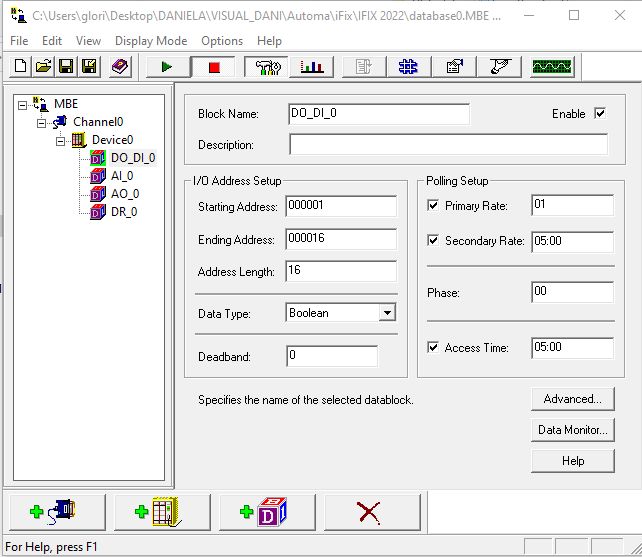
\includegraphics[scale=0.6]{mbe.png}
	\captionof{figure}{Configuración MBE}
	\label{fig:mbe}
\end{figure}
\begin{figure}[h]
	\centering
	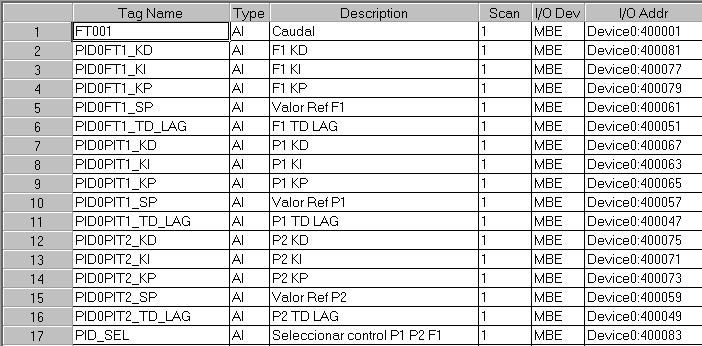
\includegraphics[scale=0.6]{database.png}
	\captionof{figure}{Configuración MBE}
	\label{fig:database}
\end{figure}


\paragraph{Pruebas mediante ModSim}
Para realizar pruebas intermedias antes de unir SCADA con el programa del PLC se utilizó el software ModSim, dónde se generó los distintos mapas de memoria utilizados para modificar variables y observar el correcto funcionamiento de distintos elementos en el SCADA.

\begin{figure}[htb]
	\centering
	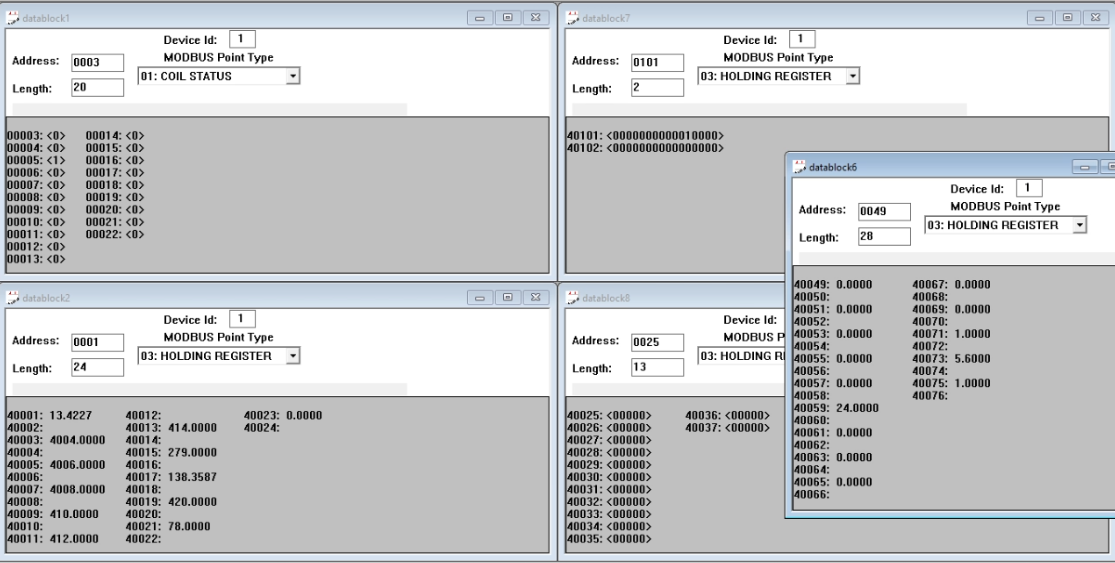
\includegraphics[width=0.9\linewidth]{modsim1.png}
	\captionof{figure}{ModSim}
	\label{fig:modsim1}
\end{figure}



\subsubsection{Alarmas y enclaves}
Dentro de la pantalla principal es posible observar el alarmero. El la tabla 
\fcolorbox{red}{yellow}{poner nombre tabla} se observa el diagrama causa efecto.

%Please add the following packages if necessary:
%\usepackage{booktabs, multirow} % for borders and merged ranges
%\usepackage{soul}% for underlines
%\usepackage[table]{xcolor} % for cell colors
%\usepackage{changepage,threeparttable} % for wide tables
%If the table is too wide, replace \begin{table}[!htp]...\end{table} with
%\begin{adjustwidth}{-2.5 cm}{-2.5 cm}\centering\begin{threeparttable}[!htb]...\end{threeparttable}\end{adjustwidth}
\begin{table}[!htp]\centering
	\caption{Generated by Spread-LaTeX}\label{tab: }
	\scriptsize
	\begin{tabular}{|l|r|r|r|r|r|r|r|r|r|r|r|r|r|r|r|r|r|}\toprule
		\multirow{2}{*}{\textbf{TAG INSTRUMENTO}} &\multirow{2}{*}{\textbf{SERVICIO}} &\multirow{2}{*}{\textbf{UNIDADES}} &\multicolumn{2}{c}{\textbf{RANGO}} &\multicolumn{4}{c}{\textbf{ALARMAS}} &\multicolumn{5}{c}{\textbf{ENCLAVAMIENTO}} &\textbf{EFECTO} &\multirow{2}{*}{\textbf{PROPOSITO DE ALARMA}} &\multirow{2}{*}{\textbf{CONSECUENCIA DE LA NO ACCION}} \\  \hline
		& & &\textbf{MIN} &\textbf{MAX} &\textbf{HI-HI} &\textbf{HI} &\textbf{LO} &\textbf{LO-LO} &\textbf{DELAY} &\textbf{HI-HI} &\textbf{HI} &\textbf{LO} &\textbf{LO-LO} &\textbf{VSD} & & \\  \hline
		\textbf{TT001} &\multirow{2}{*}{Temperatura} &\multirow{2}{*}{°C} &\multirow{2}{*}{} &\multirow{2}{*}{} & & &50 & & & & & & & &Informar alta temperatura del motor & \\  \hline
		\textbf{TT001} & & & & &70 & & & & &70 & & & &P &Informar muy alta temperatura del motor &Daño al bobinado \\  \hline
		\textbf{PIT001} &\multirow{2}{*}{Pre1} &\multirow{2}{*}{mbar} &\multirow{2}{*}{-1000} &\multirow{2}{*}{4000} &700 & & & & &700 & & & &P &Informar alta presión en cañería &Daño a bomba \\  \hline
		\textbf{PIT001} & & & & & & & & & & & & &<-1 &P &Informar desconexión PIT001 & \\  \hline
		\textbf{PIT002} &Pre2 &mbar &-1000 &4000 & & & & & & & & &<-1 &P &Informar desconexión PIT002 & \\  \hline
		\textbf{FT001} &Caudal &l/min &0 &60 & & &<0.5 & &30s & & &<0.5 & &P &Informar bajo flujo &Daño a bomba \\  \hline
		\textbf{VSD\_SC001} &Velocidad &rpm &0 &3600 &<200 & & & & &<200 & & & &P &Informar baja velocidad &Daño a motor \\  \hline
		\bottomrule
	\end{tabular}
\end{table}


\subsubsection{iHistorian}
\begin{figure}[htb]
	\centering
	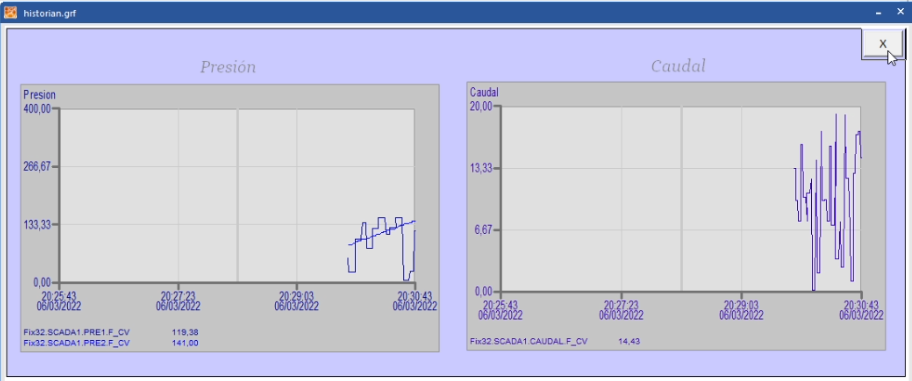
\includegraphics[scale=0.5]{scada3.png}
	\captionof{figure}{Pantalla SCADA}
	\label{fig:scada3}
\end{figure}

